\section{植物与水分}

\subsection{概述}

\subsubsection{水在植物体内的存在形式}

组织含水量的变化受植物种类、器官类型、不同生境的影响。通常生命活动较旺盛的组织含水量较高。

植物体内的水分为束缚水(结合水)和自由水两类:

\begin{description}
	\item[束缚水] 靠近蛋白质胶粒而被吸附的水分,不起溶剂作用,与抗逆性相关。
	\item[结合水] 可自由流动,起溶剂作用,与代谢强度有关。
\end{description}

\subsubsection{细胞间的水分交换}

细胞间存在两侧水势差时,水分子的运动包括:
\begin{description}
	\item[水分子的跨膜扩散] 由浓度梯度推动的,水分子直接跨过细胞膜的过程。
	\item[通过水孔蛋白的集流] 由水势差推动的,通过水孔蛋白介导的跨膜过程。
\end{description}

\paragraph{水孔蛋白}

水孔蛋白的单体由6次跨膜的$\upalpha$螺旋围成一个通道,4个单体组成一个水孔蛋白。水孔蛋白中研究最多的两类是质膜内在蛋白(PIP)和液泡膜内在蛋白(TIP)。

水孔蛋白的表达有以下特点:
\begin{description}
	\item[时空性] 发育中的组织表达量高;根尖表达量比成熟区高;TIP和PIP在根中比叶片中表达量高。
	\item[日夜节律性] 白天蒸腾强烈时表达量更高。
\end{description}

\subsection{水势}

\subsubsection{水势的计算}

水势由压力势($\psi_{\text{p}}$)、渗透势($\psi_{\uppi}$)、衬质势($\psi_{\text{m}}$)三部分组成。即\[\psi_{\text{w}}=\psi_{\text{p}}+\psi_{\uppi}+\psi_{\text{m}}\]

\begin{description}
	\item[压力势] 植物细胞吸水产生膨压,细胞壁因此产生的反作用力可阻碍吸水,这就是压力势。正常植物细胞内$\psi_{\text{p}}<0$,因为细胞壁挤压原生质体阻碍吸水;蒸腾作用下可出现$\psi_{\text{p}}>0$
	\item[渗透势] 体系内水溶质颗粒的存在导致的水势改变量,又称溶质势。$\psi_{\uppi}\approx-i\alpha CRT$,其中:
	\begin{description}
		\item[i] 溶质的范特霍夫系数,即溶质解离成几个部分,非电解质$i=1$;
		\item[$\alpha$] 溶质颗粒的活度系数,根据实验测得;
		\item[$C$] 溶质颗粒的摩尔浓度;
		\item[$R$] 理想气体常数;
		\item[$T$] 绝对温度,单位是开;
	\end{description}
	\item[衬质势] 亲水物质表面对水的吸附作用,在有大液泡的细胞内,衬质势常可忽略。
\end{description}

\begin{qj}[:植物细胞水势变化]
	常有题目考察: 把细胞放进某溶液中,问细胞内水势如何变化。答案是:若该溶液比细胞内水势高,则细胞内水势、渗透势、压力势都变高;反之则变低。概括为:“\textbf{高就高,低就低}”。
\end{qj}

\subsubsection{小液流法测定水势}

把植物组织(如叶)浸泡在不同浓度的蔗糖溶液当中,会出现以下情况:
\begin{itemize}
	\item 植物水势较高,则植物失水、溶液得水,溶液密度下降,植物下沉;
	\item 植物水势较低,则植物得水、溶液失水,溶液密度上升,植物上升;
	\item 植物水势等于溶液水势,则植物不动。
\end{itemize}



\section{光合作用}

\subsection{光合色素}

\subsubsection{光合色素的化学特性}

高等植物的光合色素有两类:类胡萝卜素和叶绿素,排列在类囊体膜上。

\paragraph{叶绿素}

叶绿素主要分为叶绿素a和叶绿素b两类。叶绿素a呈蓝绿色,叶绿素b呈黄绿色。它们能溶于有机溶剂。



叶绿素是叶绿酸和甲醇、叶绿醇发生酯化反应形成的。(\autoref{fig:cholorophyll})

\begin{figure}[htbp]
	\centering
	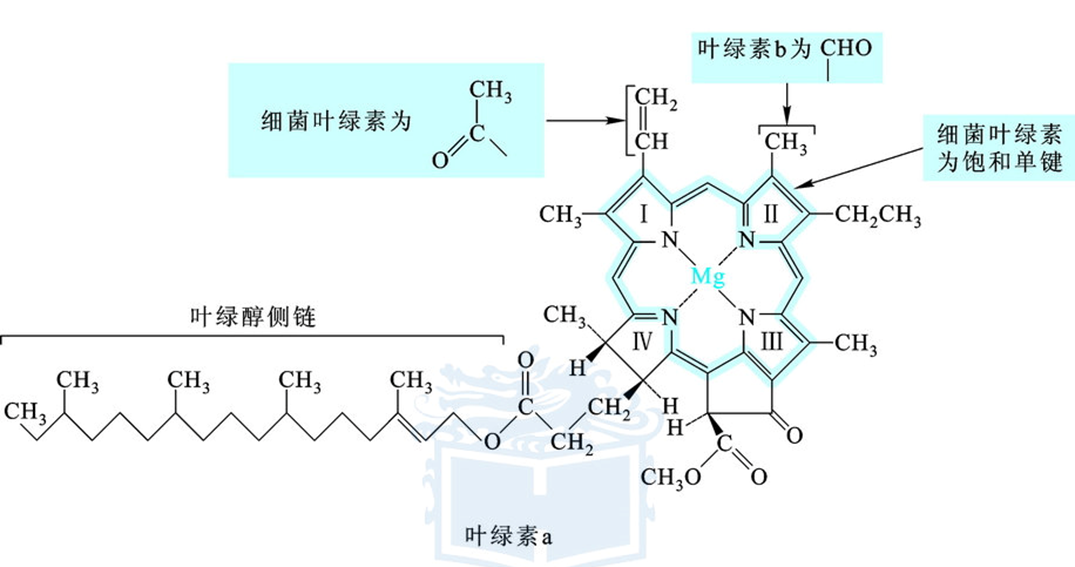
\includegraphics[width=0.9\linewidth]{Pics/叶绿素a和叶绿素b}
	\caption{叶绿素a和叶绿素b的结构}
	\label{fig:cholorophyll}
\end{figure}

叶绿素拥有亲水的金属卟啉环“头部”和疏水的叶绿醇“尾巴”。疏水的尾巴可以把叶绿素固定在类囊体膜上,亲水的头部有利于和蛋白质结合。

绝大部分叶绿素a分子和全部叶绿素b分子承担收集和传递光能的功能。少数特殊叶绿素a对承担把光能转换为化学能的功能。

\paragraph{类胡萝卜素}

叶绿体中的类胡萝卜素主要有叶黄素和$\beta$-胡萝卜素两种。叶黄素是胡萝卜素衍生的醇类。它们是重要的抗氧化剂。叶黄素呈黄色,类胡萝卜素呈橙黄色。

类胡萝卜素也有传递光能的作用,还可保护光合机构免受过剩光能伤害,如叶黄素循环。

\subsubsection{光合色素的光学特性}

\paragraph{两个吸光强区}

叶绿素主要吸收红光和蓝紫光。叶片的反射光和透射光都是绿色,叶绿素溶液也呈绿色。叶绿素溶液的荧光是红色的。(\autoref{fig:yelvsurongye})

\begin{figure}[htbp]
	\centering
	\begin{subfigure}{0.45\textwidth}
		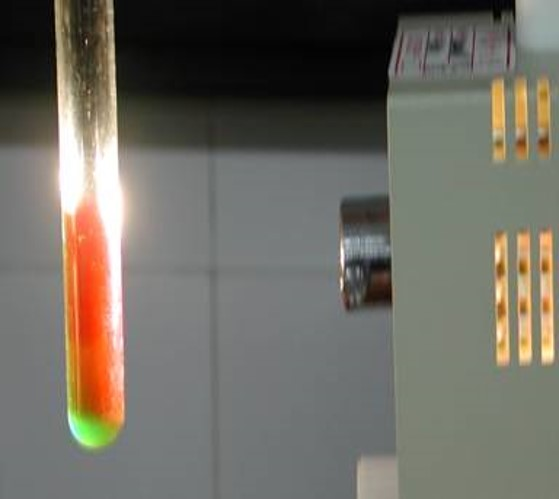
\includegraphics[width=\linewidth]{叶绿素溶液2}
	\end{subfigure}
	\hfill
	\begin{subfigure}{0.45\textwidth}
		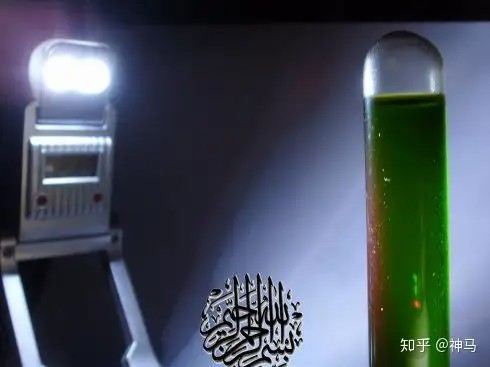
\includegraphics[width=\linewidth]{叶绿素溶液3}
	\end{subfigure}
	\caption{叶绿素溶液的透射光和反射光}
	\label{fig:yelvsurongye}
\end{figure}


类胡萝卜素主要吸收蓝紫光,不吸收红光。

\paragraph{激发态}

叶绿素分子吸收光能后,就由基态上升为激发态。激发态不稳定,停留时间非常短,以后就迅速向低能状态转变。转变的途径有:(\autoref{fig:yelvsu_light_absorb})
\begin{itemize}
	\item 以热的形式回到基态;
	\item 以荧光或磷光返回基态。荧光是从第一单线态返回时发出的光,磷光是由第一三线态返回时发出的光。磷光寿命更长。
	\item 激发态的叶绿素参与能量转移,迅速传递光能。
\end{itemize}

\begin{figure}[htbp]
	\centering
	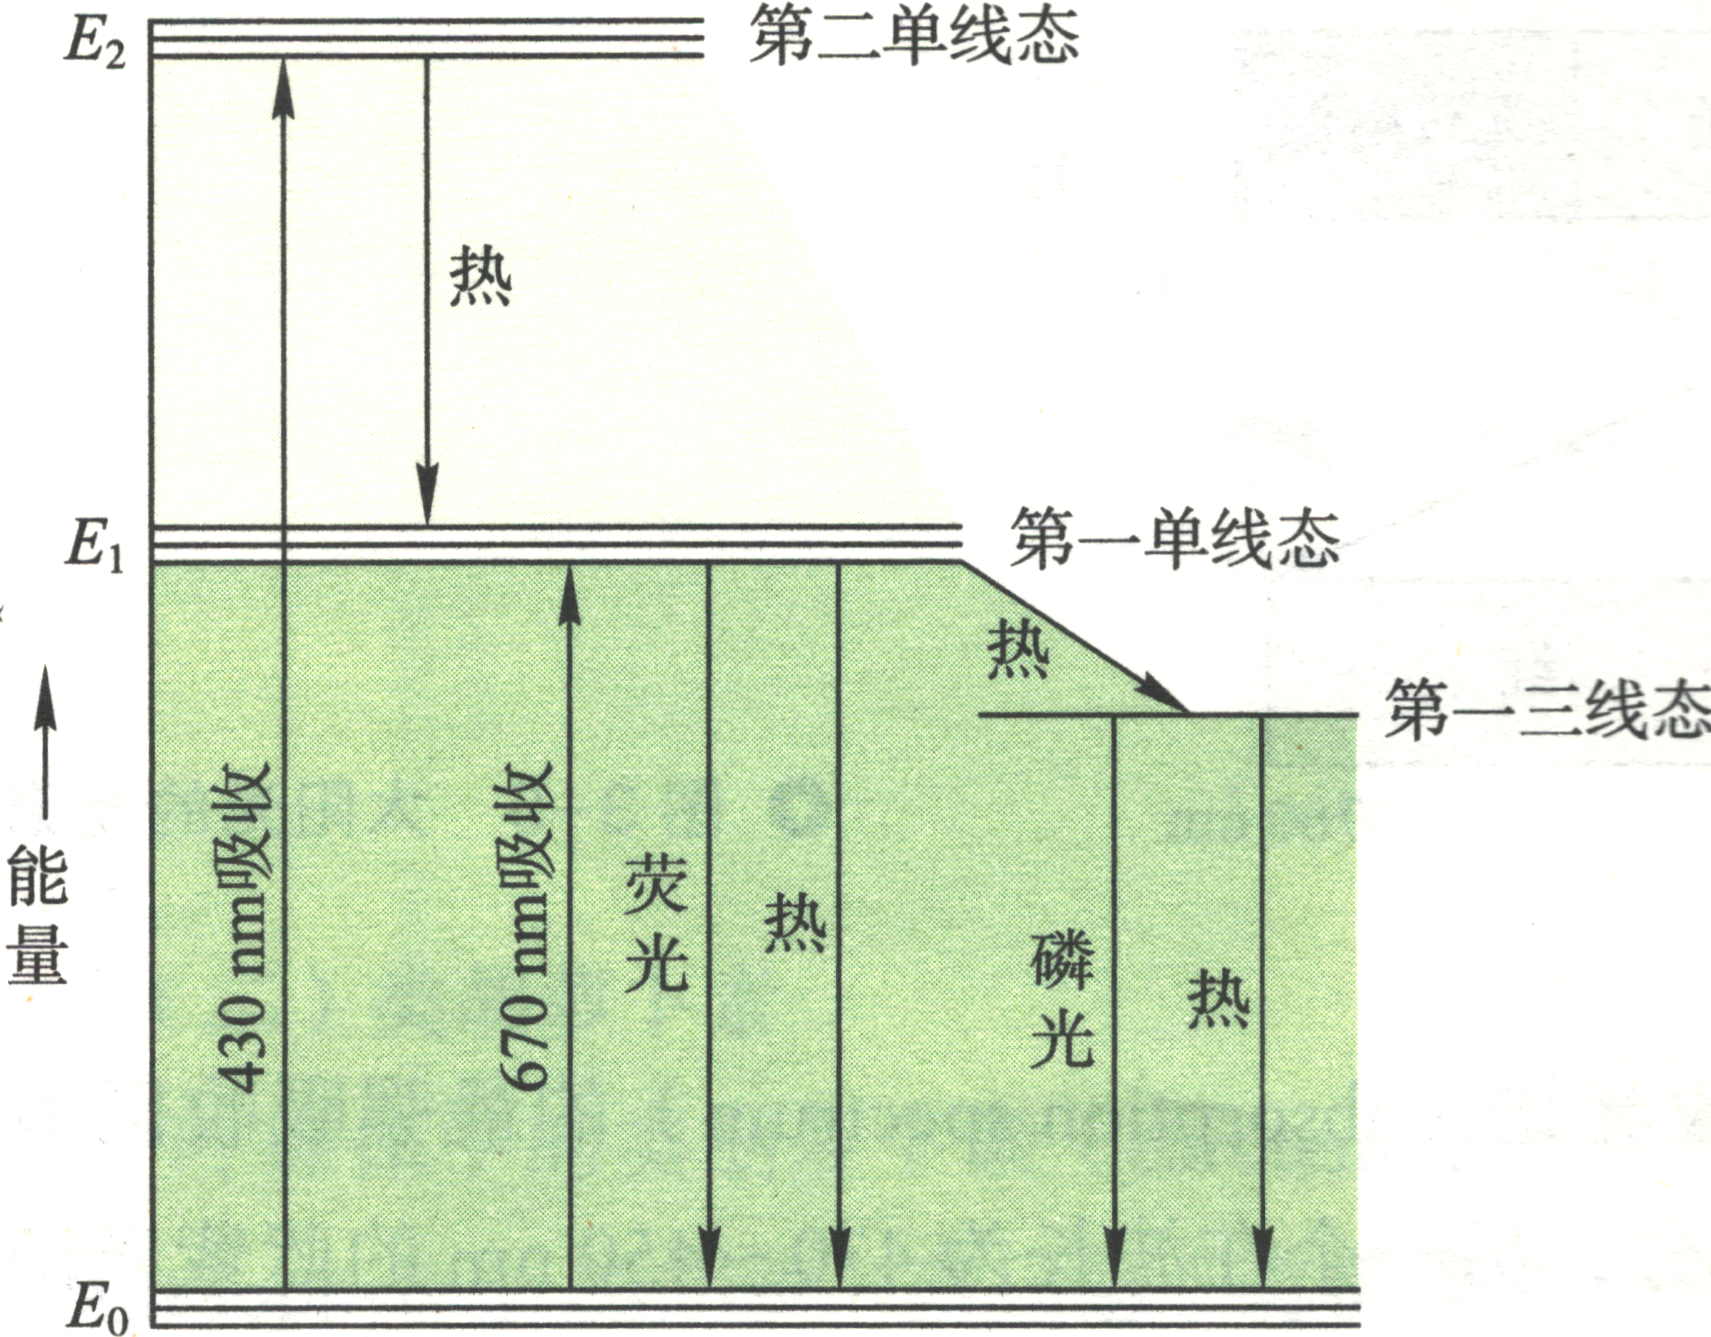
\includegraphics{叶绿素吸收光之后的能量转变}
	\caption{叶绿素吸收光之后的能量转变}
	\label{fig:yelvsu_light_absorb}
\end{figure}


\subsubsection{叶绿素的合成和降解}

\paragraph{叶绿素的合成}

叶绿素的前体是谷氨酸。反应分为四个阶段:
\begin{enumerate}
	\item 谷氨酸$\longrightarrow$5-氨基酮戊酸$\longrightarrow$卟胆原;
	\item 4个卟胆原$\longrightarrow$原卟啉IX$\xrightarrow{\ce{Mg^{2+}}}$Mg原卟啉$\longrightarrow$单乙烯基原叶绿素酯a;
	\item 单乙烯基原叶绿素酯a$\xrightarrow{\text{NADPH、光}}$叶绿素酯a;
	\item 叶绿素酯a$\xrightarrow{植醇尾巴}$叶绿素a。
\end{enumerate}

叶绿素b是由叶绿素a演变来的。

\paragraph{叶绿素的降解}

叶绿素b$\longrightarrow$叶绿素a$\longrightarrow$脱植基叶绿素a$\longrightarrow$脱镁叶绿素a$\longrightarrow$水溶性无色产物,进入液泡。

\paragraph{植物的叶色}

植物的叶色是各种色素的综合表现。

\begin{itemize}
	\item 正常植物呈绿色:叶绿素比类胡萝卜素多;
	\item 秋天呈红色:气温降低,叶绿素分解,显示出类胡萝卜素的颜色。
	\item 枫树变红:积累糖分御寒,利用糖分合成红色的花色素苷。
\end{itemize}

因此,影响光合色素合成的因素可以影响植物的叶色:

\begin{description}
	\item[光] 叶绿素合成需要光。一般植物在黑暗中无法合成叶绿素,导致黄化。
	\item[温度] 温度影响酶的活性。
	\item[矿质元素] 氮和镁是组成叶绿素的元素。一些金属离子是叶绿素合成有关酶的活化剂。
\end{description}

\subsection{光合作用过程}





\subsubsection{碳同化}

\paragraph{C$_{3}$途径}

\paragraph{C$_{4}$途径}

\subsection{光呼吸}

\begin{figure}[htbp]
	\centering
	\includegraphics{光呼吸}
	\caption{光呼吸}
	\label{fig:光呼吸}
\end{figure}



\section{植物同化物的运输}

\subsection{概述:运输的途径和方向}

\subsubsection{运输途径}

\begin{description}
	\item[短距离运输] 同化物在细胞内或细胞之间的运输;
	\item[长距离运输] 同化物经维管系统,从源到库的运输。
\end{description}

\paragraph{短距离运输}